\documentclass[../report.tex]{subfiles}
\begin{document}
	\begin{frame}
    	\frametitle{Challenge problem - A}
    	\begin{table}[!htb]
        \centering
        \begin{tabular}{ c m{5cm} }
        
            \begin{minipage}{.45\textwidth}
            \frame{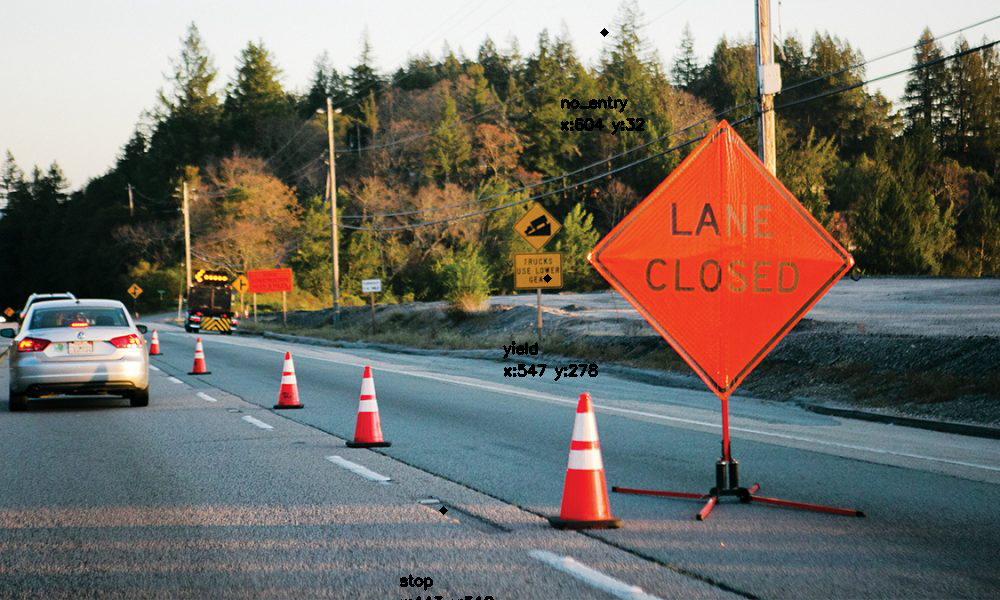
\includegraphics[keepaspectratio,height=0.7\textheight,width=1\textwidth]{ps2-5-a-1}}
                \captionof{figure}{ps2-5-a-1}
            \end{minipage}
            &
            \begin{minipage}{.45\textwidth}
                Coordinates and Name: \\
                misdetected yeild sign: (547 278) \\

            \end{minipage}
        
        \end{tabular}
        \end{table}
    \end{frame}

    \begin{frame}
    	\frametitle{Challenge problem - A}
    	\begin{table}[!htb]
        \centering
        \begin{tabular}{ c m{5cm} }
        
            \begin{minipage}{.45\textwidth}
            \frame{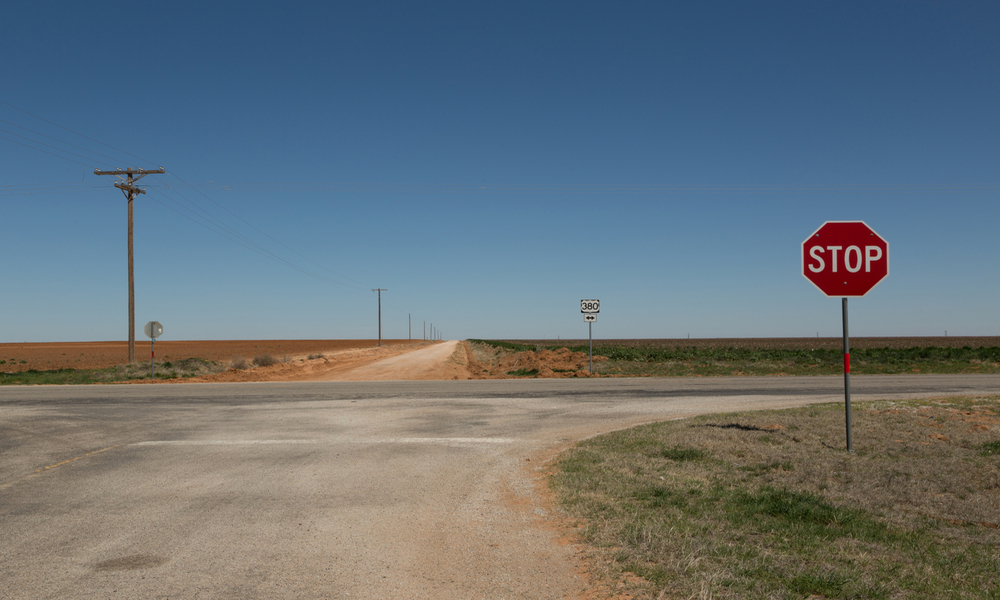
\includegraphics[keepaspectratio,height=0.7\textheight,width=1\textwidth]{ps2-5-a-2}}
                \captionof{figure}{ps2-5-a-2}
            \end{minipage}
            &
            \begin{minipage}{.45\textwidth}
                Coordinates and Name: \\
                Failed to detect \\

            \end{minipage}
        
        \end{tabular}
        \end{table}
    \end{frame}

    \begin{frame}
    	\frametitle{Challenge problem - A}
    	\begin{table}[!htb]
        \centering
        \begin{tabular}{ c m{5cm} }
        
            \begin{minipage}{.45\textwidth}
            \frame{
\includegraphics[keepaspectratio,height=0.7\textheight,width=1\textwidth]{ps2-5-a-3}}
                \captionof{figure}{ps2-5-a-3}
            \end{minipage}
            &
            \begin{minipage}{.45\textwidth}
                Coordinates and Name: \\
                misdetected stop sign (926, 222) \\

            \end{minipage}
        
        \end{tabular}
        \end{table}
    \end{frame}

    \begin{frame}
    	\frametitle{Challenge problem - B}
    	\begin{table}[!htb]
        \centering
        \begin{tabular}{ c m{5cm} }
        
            \begin{minipage}{.45\textwidth}
            \frame{
\includegraphics[keepaspectratio,height=0.7\textheight,width=1\textwidth]{ps2-5-b-1}}
                \captionof{figure}{ps2-5-b-1}
            \end{minipage}
            &
            \begin{minipage}{.45\textwidth}
                Coordinates and Name: \\
                No Entry: (-1, -1) \\
No Entry: (-1, -1) \\
            \end{minipage}
        
        \end{tabular}
        \end{table}
    \end{frame}

    \begin{frame}
    	\frametitle{Challenge problem - B}
    	\begin{table}[!htb]
        \centering
        \begin{tabular}{ c m{5cm} }
        
            \begin{minipage}{.45\textwidth}
            \frame{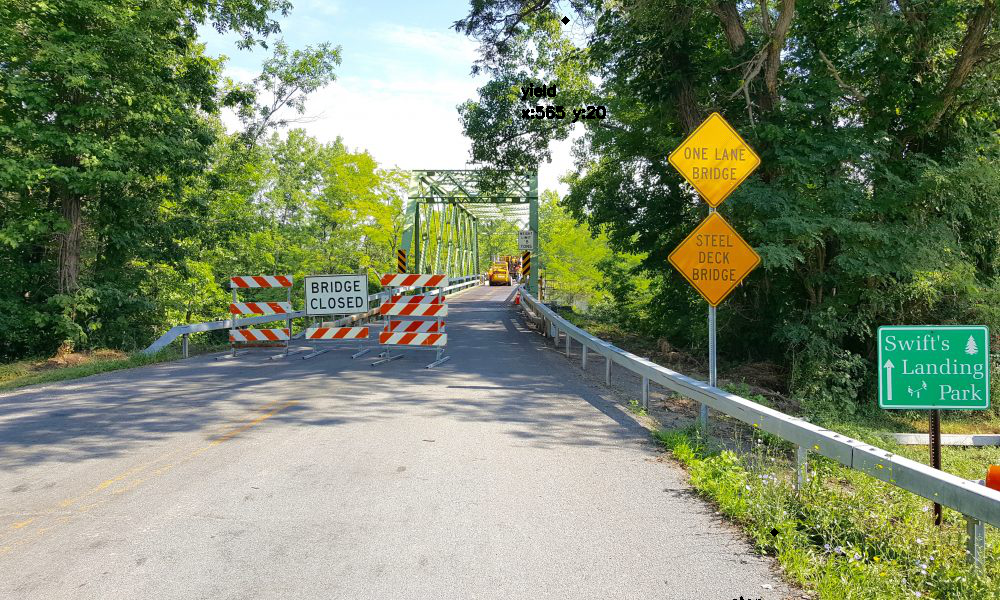
\includegraphics[keepaspectratio,height=0.7\textheight,width=1\textwidth]{ps2-5-b-2}}
                \captionof{figure}{ps2-5-b-2}
            \end{minipage}
            &
            \begin{minipage}{.45\textwidth}
                Coordinates and Name: \\
                No Entry: (-1, -1) \\
No Entry: (-1, -1) \\
            \end{minipage}
        
        \end{tabular}
        \end{table}
    \end{frame}

    \begin{frame}
    	\frametitle{Challenge problem - B}
    	\begin{table}[!htb]
        \centering
        \begin{tabular}{ c m{5cm} }
        
            \begin{minipage}{.45\textwidth}
            \frame{
\includegraphics[keepaspectratio,height=0.7\textheight,width=1\textwidth]{ps2-5-b-3}}
                \captionof{figure}{ps2-5-b-3}
            \end{minipage}
            &
            \begin{minipage}{.45\textwidth}
                Coordinates and Name: \\
                No Entry: (-1, -1) \\
No Entry: (-1, -1) \\
            \end{minipage}
        
        \end{tabular}
        \end{table}
    \end{frame}
	
	\begin{frame}[t]
		\frametitle{Challenge problem - Text}
		
		\begin{normalsize}
			\begin{itemize}
				\setlength\itemsep{1em}\fontsize{6pt}{6pt}
				
				\item[] \textbf{Describe what you had to do to adapt your code for this task. How does the difference between simulated and real-world images affect your method? If you used other functions/methods, explain why that was better (or why your previous implementation did not work)}

				\item[] {\selectfont\textcolor{blue}{5c answer here \\
5c answer here \\
5c answer here \\
5c answer here \\}}

			\end{itemize}
		\end{normalsize}
		
	\end{frame}

\end{document}